\documentclass[11pt, oneside]{article}   	% use "amsart" instead of "article" for AMSLaTeX format
\usepackage{geometry}                		% See geometry.pdf to learn the layout options. There are lots.
\geometry{letterpaper}                   		% ... or a4paper or a5paper or ... 
%\geometry{landscape}                		% Activate for rotated page geometry
%\usepackage[parfill]{parskip}    		% Activate to begin paragraphs with an empty line rather than an indent
\usepackage{graphicx}				% Use pdf, png, jpg, or eps§ with pdflatex; use eps in DVI mode

								% TeX will automatically convert eps --> pdf in pdflatex		
\usepackage{amssymb}

\usepackage{amsmath}
\usepackage[mathscr]{euscript}
\usepackage[shortlabels]{enumitem}

\newcommand{\R}{\mathbb{R}}
\newcommand{\Z}{\mathbb{Z}}
\newcommand{\Q}{\mathbb{Q}}
\newcommand{\C}{\mathbb{C}}
\newcommand{\F}{\mathbb{F}}
\newcommand{\bb}[1]{\mathbb{#1}}
\newcommand{\scr}[1]{\mathscr{#1}}
\newcommand{\tand}{\text{ and }}
\newcommand{\tor}{\text{ or }}
\newcommand{\twhere}{\text{ where }}
\newcommand{\tfor}{\text{ for }}
\newcommand{\st}{\mid}
\newcommand{\qed}{\begin{center}
$\square$
\end{center}}
\newcommand{\nullset}{\varnothing}
\newcommand{\set}[1]{\{ #1 \}}

%SetFonts

%SetFonts


\title{Selected Exercises \S27 \& \S30}
\author{Colton Kinstley}
%\date{}							% Activate to display a given date or no date

\begin{document}
\maketitle

\section*{Question 2}
Let $X$ be a metric space with metric d; let $A \subset X$ be nonempty.
\begin{enumerate}[(a)]
\item
Show that \dots
\item
Show that if $A$ is compact, $d(x,A) = d(x,a) $ for some $a \in A$.
\item
Define the \dots
\item
Assume that $A$ is compact; let $U$ be and open set containing $A$. Show that some $\epsilon$-neighborhood of $A$ is contained in $U$. 
\item
Show the result in (d) need not hold if $A$ is closed but not compact.
\end{enumerate}

\subsection*{Solution (b)}
Since $d: X \times X \to \R$ is continuous its restriction to $X \times A$ is also continuous. Fixing $x \in X$ we minimize the continuous function $d \big \vert_A:A \to \R$ to obtain the value of $d(x,A)$. Because $A$ is compact we can apply theorem 27.4 [Munkres]  (the extreme value theorem) to obtain $c \in A$ such that $d(x,c) \leq d(x,a)$ for all $a \in A$. Hence the infimum in the definition of $d(x,A)$ is in fact obtained by $c \in A$ and $d(x,A) = d(x,c)$.

\subsection*{Solution (d)}
Since $U$ is an open set in $X$ we have that for each $a \in A \subset U$ there is a basis element $B_d(a,\epsilon)$ with $\epsilon$ depending on $a$ that is a subset of $U$. This set of balls forms an open cover of $A$ and because $A$ is compact there exists $\set{B_d(a_i,\epsilon_i)}_{i=1}^n$ a finite subcover. Let $\epsilon = \min_{i=1, \dots, n} \set{ \epsilon_i}$ then we have $U(A,\epsilon) = \bigcup_i B_d(a_i,\epsilon_i) \subset U$, since for each $i = 1, \dots, n$

\[
B_d(a_i,\epsilon) \subset B_d(a_i,\epsilon_i) \subset U.
\]

\subsection*{Solution (e)}
Take $(X,d)$ = $\R \times \R$ with the usual metric. Let $A = [1,\infty) \times \set{0}$. Then an open set containing $A$ is $U = (0,\infty) \times \R \cap \set{(x,y) \st x>0, -e^{-x} < y < e^{-x}}$. 

\begin{figure}[h]
\caption{Visualization of A, U and U(A,$\epsilon$)}
\centering
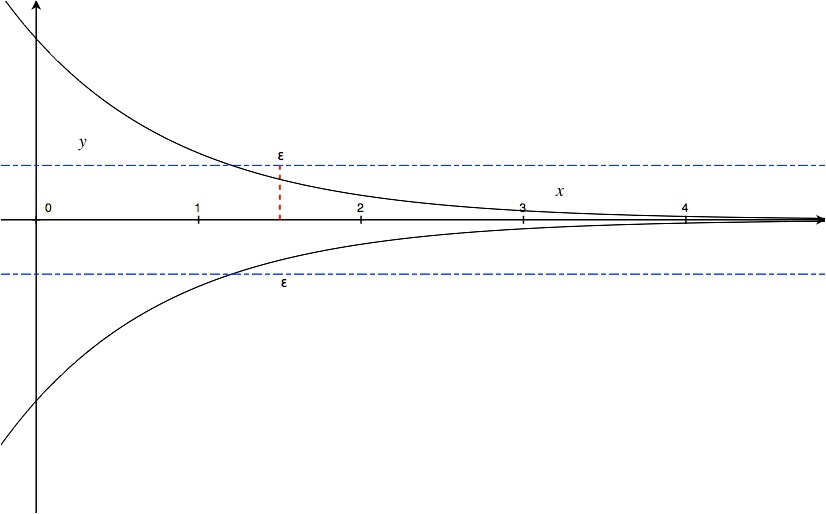
\includegraphics[scale=.5]{graph}
\end{figure}

Suppose that there were an $\epsilon > 0$ such that $U(A,\epsilon) \subset U$. Then the point $(1-\ln{\epsilon}, \epsilon / 2)$ would lie in $U(A,\epsilon)$ but if $U(A,\epsilon) \subset U$ this implies that

\begin{equation*}
\epsilon/2 < e^{-(1-\ln{\epsilon})} = \epsilon/e 
\end{equation*}
a contradiction.

\section*{Question 10}

Show that if $X$ is a countable product of spaces having countable dense subsets, then $X$ has a countable dense subset.

\subsection*{Solution}

Let $X = \prod_{i=1}^\infty X_i$ be a countable product of spaces and suppose for each $i = 1, \dots, n$ $A_i \subset X_i$ is a countable dense subset. We can show that $X$ has a countable dense subset by constructing one. Let $A = \prod_{i=1}^\infty A_i$, we will show that $A$ is a countable dense subset of $X$. That $A$ is countable is clear as it is the countable product of countable sets. To see that $A$ is dense in $X$ we apply theorem 19.5 [Munkres] to see that

\begin{equation*}
\bar{A} = \overline{\prod_iA_i} = \prod_i \bar{A_i} = \prod_i X_i = X.
\end{equation*}





















































\end{document}
